\documentclass[a4paper]{D:/repositories/MyDGP/latex/PaperReadingLog}
\usepackage{caption}
\usepackage{overpic}
\usepackage{float}

\usepackage{enumitem} 
\usepackage{amsfonts,amssymb,amsmath}
\usepackage[linesnumbered,ruled,lined]{algorithm2e}%%伪代码
\usepackage{multicol}
\usepackage{wrapfig}
\setmainfont{Arial}

\begin{document}

\PaperInfo
{参数化}
{朱}
{天宇}
{}
\section{Tutte参数化}
\subsection{知识内容}
\subsubsection{LU分解}
在解方程的步骤中需要用到Eigen的LU分解功能。LU分解可以将一个矩阵分解为上三角矩阵和下三角矩阵,分解的原理很简单:通过高斯消元操作可以将矩阵消元为上三角矩阵,而相应的初等变化步骤可以记录为一个下三角矩阵。\href{https://blog.csdn.net/qq_40688707/article/details/89256737}{详细信息}

\subsection{代码细节}
\subsubsection{输入预处理}
在读入网格后,需要确认网格是一个亏格为0的开网格。之后,将网格的边界点映射到一个圆上。

首先,遍历网格所有顶点,获取边界顶点的数量。之后,随机选择一个顶点为起点$st$。之后,对于点$m$,寻找这样的相邻点$n$:\begin{itemize}
    \item $n$是一个边界点
    \item 边$(m,n)$是一个边界边
\end{itemize}
寻找相邻点的操作通过自定义函数find\_neighbour完成。

从起点$st$开始,依次寻找满足条件的相邻点,之后将这些点\textbf{有序的}存入边界点数组Bnd\_v\_inorder中,直到返回起点为止。此时检测边界点数组的size和总的边界点数量是否相同,如果不同则说明网格并非一个disk topology的。返回错误。

\subsubsection{构建矩阵和解方程}
\paragraph{构建矩阵}
使用Eigen来定义矩阵。使用$\mathrm{A}_{n\times n}$用于存放等式的参数,其中$n$是网格顶点的数量。使用矩阵$b_{n\times 2}$用于存放等号右边的数值,其两列分别表示$u,v$的值。

对于边界点$VB$来说,其在参数化结果中的顶点位置是已知的,因而其在$\mathrm{A}$的对应行$v_{index}$,仅有第$v_{index}$列的数值为1。而在$b$的第$v_{index}$行,其两列数值分别为边界点的$uv$坐标。这表示在方程等式中,边界点的值就等于$b$的值。

对于内部点$VI$来说,其值等于其1-邻域数值的加权平均。因而等式右边的值为0,而左边有2种写法,一种是将邻域顶点对应的列的值写成$\frac{1}{n}$,将$VI$对应的列值记为$-1$;另一种是将邻域对应的列值记为1,将$VI$对应的列的值记为$-n$。\textbf{推荐使用后一种写法}。这样做矩阵$\mathrm{A}$就是对称的矩阵,有专门的计算方法。

\paragraph{解方程}
使用Eigen库的SparseLU的solver来求解。LU分解的原理在上面。

\subsubsection{后处理}
根据上文定义,令$X=\mathrm{A}^{-1}\times b$,$X_{n\times 2}$就是参数化结果的UV坐标。将$X$每行的值分别作为矩阵顶点的位置值即可。

\subsection{最终结果}
这里展示一个输入网格以及其对应的结果。
\begin{figure}[H]%使用H表示Here,不对图片排版!
    \centering
    \begin{overpic}[width=0.8\linewidth]{fig/1.png}
    \end{overpic}
    \vspace{-3.5mm}
    \caption{Tutte参数化结果}
    \vspace{2mm}
\end{figure}

\section{LSCM}
LSCM,Least squares conformal maps,最小二乘的共形映射。可以获得输入网格的一个共形映射。\textbf{共形就是相似},参数化后的三角面片和参数化前的三角面片要尽可能的相似。LSCM提出了一种度量三角面片相似性的能量,通过求这个能量的最小值,就可以获得一个共形参数化的结果。

\subsection{知识内容}

\subsubsection{Jacobian矩阵}
三角形从一个形状到另一个形状的变化可以通过Jacobian矩阵来描述。Jacobian矩阵的定义如图:

\begin{figure}[H]%使用H表示Here,不对图片排版!
    \centering
    \begin{overpic}[width=0.8\linewidth]{fig/2.png}
    \end{overpic}
    \vspace{-3.5mm}
    \caption{Jacobian矩阵}
    \vspace{2mm}
\end{figure}

\subsubsection{共形能量}
根据图中描述,给一个三角形乘上一个Jacobian矩阵,就可以得到一个形变后的三角形。\textbf{如果希望每个面片在变形前后保持形状不变,那么其Jacobian矩阵最好是一个旋转矩阵。}对于一个二维的旋转矩阵,其应该类似于这样:\href{https://www.cnblogs.com/suerchen/p/4833381.html}{(绘制矩阵的方法)}
$$
\begin{pmatrix}
    \cos\theta & -\sin\theta \\ 
    \sin\theta & \cos\theta
\end{pmatrix}
$$

而Jacobian矩阵的写法是
$$J=
\begin{pmatrix}
    \frac{\partial u}{\partial x} & \frac{\partial u}{\partial y} \\
    \frac{\partial v}{\partial x} & \frac{\partial v}{\partial y}
\end{pmatrix}
$$

要使得Jacobian矩阵类似于旋转矩阵,就需要令$\frac{\partial u}{\partial x}=\frac{\partial v}{\partial y},\frac{\partial u}{\partial y}=-\frac{\partial v}{\partial x}$。据此可以定义二次能量:
$$
E_{LSCM}=\sum_t A_t((\frac{\partial u}{\partial x}-\frac{\partial v}{\partial y})^2+(\frac{\partial u}{\partial y}+\frac{\partial v}{\partial x})^2)
$$
优化这个能量即可。这个这个能量是旋转不变的。然而,根据式子可以发现,这个能量的最小值不唯一,\textbf{所以还需要固定两个顶点的位置。}

\subsubsection{能量优化}
该能量是一个二次能量,因此可以通过分别求偏导数直接获得最小值。

\subsection{代码细节}
\subsubsection{输入参数}
LSCM需要固定两个顶点,所以算法的输入参数为网格名和两个顶点。
\subsubsection{构建矩阵}
能量$E_{LSCM}$是由2n个未知数构成的一个很长的等式,这里n是顶点的数量,每个点有$uv$坐标所以一共2n个。对这2n个未知数分别求偏导,就可以得到2n个等式。另外,需要固定2个顶点的位置,所以还会有4个等式。所以一共是2n+4个等式。

等式的系数通过Jacobian矩阵数值来确定,就是那个2x3的矩阵。

因此,使用矩阵$A_{2n+4,2n+4}$来记录方程组的所有系数,使用$b_{2n+4}$记录方程组右边的数值。

由于$A$是稀疏矩阵,所以使用Eigen的稀疏矩阵功能来表示,具体写法见代码。

\subsubsection{解方程}
由于$A$非对称,使用Eigen库的SparseLU的solver来求解。

\subsection{后处理}
根据上文定义,令$X=\mathrm{A}^{-1}\times b$,$X_{n\times 2}$就是参数化结果的UV坐标。将$X$每行的值分别作为矩阵顶点的位置值即可。

\subsection{最终结果}
这里展示一个输入网格以及其对应的结果。
\begin{figure}[H]%使用H表示Here,不对图片排版!
    \centering
    \begin{overpic}[width=0.8\linewidth]{fig/3.png}
    \end{overpic}
    \vspace{-3.5mm}
    \caption{LSCM参数化结果}
    \vspace{2mm}
\end{figure}

\section{ABF参数化}
ABF,Angle-Based Flattening,保持角度的Flattening。这个方法的想法比较直观:依旧希望参数化后的三角形和之前的三角形的角度相同。LSCM通过三角形的Jacobian矩阵来度量相似的程度,而ABF则设法直接保持角度。

\subsection{算法描述}
\subsubsection{能量项}
ABF方法的能量项为:
$$
E_{ABF}=\sum_t\sum_{i=1}^3\omega_i^t(\alpha_i^t-\beta_i^t)^2
$$
这其中,$t$是三角面片,$\beta$是输入网格的三角形的每个角的度数,是已知量;$\alpha$是需要求的参数化后的三角形的角度;$\omega$是和$\beta$相关的量。详细的定义为\href{https://blog.csdn.net/miao0967020148/article/details/78712811}{(如何画大括号?)}
    $$ \beta_i^t=\left\{
\begin{aligned}
\frac{\widetilde{\beta_i^t}\cdot 2\pi}{\sum_i\widetilde{\beta_i^t}}, Interior\ Vertex \\
\widetilde{\beta_i^t},Boundary\ Vertex\\
\end{aligned}
\right.
$$
$$
\omega_i^t=(\beta_i^t)^{-2}
$$
\subsubsection{约束项}
此外,参数化后的三角形还应当满足如下\textbf{约束}。\begin{enumerate}
    \item 所有的角都应该是大于0的,$\alpha_i^t>0$。在代码中本项不纳入考虑。
    \item 三角形内角和为$\pi$,$\alpha_1^t+\alpha_2^t+\alpha_3^t=\pi$
    \item 一个顶点一邻域的角度之和应当为$2\pi$,$\sum_{t\in \Omega(v)}\alpha_k^t=2\pi$
    \item \textbf{重建约束}:
    $$
    \prod_{t\in \Omega(v)}\sin\alpha_{k\oplus 1}^t=    \prod_{t\in \Omega(v)}\sin\alpha_{k\ominus 1}^t
    $$
\end{enumerate}

\paragraph{重建约束}
重建约束的含义如右图所示。由于算法只关心约束角度,那么理论上三角形应当是可以放缩的。那么为了使一个点的1-邻域三角形可以完美的\textbf{咬合}。其推导过程如下:
\begin{figure}[H]%使用H表示Here,不对图片排版!
    \centering
    \begin{overpic}[width=0.8\linewidth]{fig/5.png}
    \end{overpic}
    \vspace{-3.5mm}
    \caption{重建约束的推导}
    \vspace{2mm}
\end{figure}
这项约束涉及三角函数,是\textbf{非线性的},所以需要将其取对数后泰勒展开,只保留第一项,转变成线性约束。用初始估计$\gamma$和误差项$e$来表示$\alpha,\alpha_i^t=\gamma_i^t+e_i^t$
$$
\begin{aligned}
    \log(\sin\alpha_{k\oplus 1}^t)=\log(\sin\gamma_{k\oplus 1}^t+e_{k\oplus 1}^t)\\
    =log(\sin\gamma_{k\oplus 1}^t)+e_{k\oplus 1}^t\cot\gamma_{k\oplus 1}^t    
\end{aligned}
$$
那么最终重建约束的线性形式是:
$$
\log\sin 1+e_1*\cot 1-\log\sin 2+e_2*\cot 2+\log\sin 3+e_3*\cot 3+...=0
$$
这其中,$e_i$是未知量,$\cot$是权重,$\log\sin$是等式右边的数值。

\subsubsection{从角度重建UV坐标}
\paragraph{贪婪法}
贪婪法首先选择起始边$e^1=(v_a^1,v_b^1)$,将两个顶点投影到$(0,0,0),(\lVert e^1 \lVert,0,0)$,随后将起始边压入栈$S$中。
\textbf{当$S$不为空的时候},每次从栈中取一条边$e=(v_a,v_b)$,对于每个含有该边的面$f_i=(v_a,v_b,v_c)$:\begin{itemize}
    \item 如果$f_i$被标记了,则continue
    \item 如果$v_c$未被投影,则根据$v_a,v_b,f_i$的信息,投影$v_c$。之后标记$f_i$,并且将$(v_b,v_c)$以及$(v_a,v_c)$压栈
\end{itemize}
这种做法会导致误差积累。
\paragraph{最小二乘方法}
由于三角形的三个角是已知的,那么对于其三个顶点$P_k,P_j,P_l$以及其三个角$\alpha_k,\alpha_j,\alpha_l$来说,根据正弦定理可以得到$(P_k,P_l)$与$(P_k,P_j)$的长度比值,通过旋转矩阵则可以将其中一条边旋转到另一条边的角度。如果记$M$为旋转矩阵乘以长度比值,就可以得到等式
$$
M(P_k-P_j)+P_j-P_l=0
$$
其中,M是根据正弦定理表达的长度比值乘以旋转矩阵:
$$
M=\frac{\sin \alpha_k}{\sin \alpha_l}
\begin{pmatrix}
    \cos\alpha_j & -\sin\alpha_j \\ 
    \sin\alpha_j & \cos\alpha_j
\end{pmatrix}
$$
可以将这个的平方作为约束的能量,之后求解方程,将贪婪法之中的误差均摊到各条边上。
能量记作:
$$
E=\sum_t\lVert M^t(P_k-P_j)+P_j-P_l\lVert^2
$$
当然,这么做依旧需要固定两个点的位置。
对于每一个三角面片$t$,其三个顶点$j,k,l$所对应的能量展开形式为:
$$\begin{aligned}
E&=
\lVert \begin{pmatrix}
    M_{00} & M_{01} \\ 
    M_{10} & M_{11}
\end{pmatrix}
\begin{pmatrix}
    x_k-x_j  \\ 
    y_k-y_j
\end{pmatrix}+
\begin{pmatrix}
    x_j-x_l  \\ 
    y_j-y_l
\end{pmatrix}
\lVert ^2 \\
&=\lVert
\begin{pmatrix}
    M_{00}(x_k-x_j)+M_{01}(y_k-y_j)+(x_j-x_l) \\ 
    M_{10}(x_k-x_j)+M_{11}(y_k-y_j)+(y_j-y_l)
\end{pmatrix}
\lVert^2 \\
&=(M_{00}(x_k-x_j)+M_{01}(y_k-y_j)+(x_j-x_l))^2+(M_{10}(x_k-x_j)+M_{11}(y_k-y_j)+(y_j-y_l))^2\\
&=(M_{00}x_k+(1-M_{00})x_j+M_{01}y_k-M_{01}y_j-x_l)^2+(M_{10}x_k-M_{10}x_j+M_{11}y_k+(1-M_{11})y_j-y_l)^2
\end{aligned}
$$
分别对$x_j,y_j,x_k,y_k,x_l,y_l$求偏导,可以获得\textbf{(能量有2个部分,这里上下行要相加,为了方便阅读写成这样)}
$$\begin{aligned}
    \frac{\partial E}{\partial x_j}&=\begin{array}[]{cccccc}
        2(1-M_{00})^2x_j & 2M_{00}(1-M_{00})x_k & -2(1-M_{00})x_l & -2M_{01}(1-M_{00})y_j & 2M_{01}(1-M_{00})y_k & 0 \\
        2M_{10}^2x_j & -2M_{10}^2x_k & 0 & -2M_{10}(1-M_{11})y_j & -2M_{10}M_{11}y_k & 2M_{10}y_l\\
    \end{array}\\
    \frac{\partial E}{\partial x_k}&=\begin{array}[]{cccccc}
    2M_{00}(1-M_{00})x_j & 2M_{00}^2x_k & -2M_{00}x_l & -2M_{00}M_{01}y_j& 2M_{00}M_{01}y_k & 0 \\
    -2M_{10}^2x_j & 2M_{10}^2x_k & 0 & 2M_{10}(1-M_{11})y_j& 2M_{10}M_{11}y_k & -2M_{10}y_l \\
    \end{array}\\
    \frac{\partial E}{\partial x_l}&=\begin{array}[]{cccccc}
    -2(1-M_{00})x_j & -2M_{00}x_k & 2x_l & 2M_{01}y_j& -2M_{01}y_k & 0 \\
    0 & 0 & 0 & 0& 0 & 0 \\
    \end{array}\\
    \frac{\partial E}{\partial y_j}&=\begin{array}[]{cccccc}
    -2M_{01}(1-M_{00})x_j & -2M_{01}M_{00}x_k & 2M_{01}x_l & 2M_{01}^2y_j& -2M_{01}^2y_k & 0 \\
    -2(1-M_{11})M_{10}x_j & 2(1-M_{11})M_{10}x_k & 0 & 2(1-M_{11})^2y_j& 2(1-M_{11})M_{11}y_k & -2(1-M_{11})y_l \\
    \end{array}\\
    \frac{\partial E}{\partial y_k}&=\begin{array}[]{cccccc}
        2M_{01}(1-M_{00})x_j & 2M_{01}M_{00}x_k & -2M_{01}x_l & -2M_{01}^2y_j& 2M_{01}^2y_k & 0 \\
        -2M_{10}M_{11}x_j & 2M_{10}M_{11}x_k & 0 & 2M_{11}(1-M{11})y_j& 2M_{11}^2y_k & -2M_{11} \\
    \end{array}\\
    \frac{\partial E}{\partial y_l}&=\begin{array}[]{cccccc}
        0 & 0 & 0 & 0& 0 & 0 \\
        2M_{10}x_j & -2M_{10}x_k & 0 & -2(1-M_{11})y_j& -2M_{11}y_k & 2y_l \\
    \end{array}\\
    % 0 & 0 & 0 & 0& 0 & 0 \\
    % 0 & 0 & 0 & 0& 0 & 0 \\
\end{aligned}
$$


\subsection{知识背景}
由于重构约束项的相关处理,算法以\textbf{变化前后的角度之差e}作为变量。另外,第一项约束不予以考虑,因此本问题就是一个\textbf{带有线性约束的二次能量优化},可以用\textbf{拉格朗日乘数法}来解决。

\subsubsection{拉格朗日乘数法}
可以用于求带约束的二次能量的极值。以下是一个例子:\href{http://blog.sina.com.cn/s/blog_6850cf720101a9kk.html}{(如何排版优化问题公式)}
$$
\begin{aligned}
    &\min\quad E=x_1^2+2x_2^2+3x_3^2\\
    & \begin{array}{r@{\quad}r@{}l@{\quad}l}
    s.t.&x_1+x_2&=2  \\
     &x_1+4x_3&=4&
    \end{array} .
    \end{aligned}
    $$
    
对于每一个等式约束,都在其前面加上一个$\lambda$,之后将约束也作为优化能量的一个部分,可以写成
$$
\min\quad L=x_1^2+2x_2^2+3x_3^2-\lambda_1(x_1+x_2-2)-\lambda_2(x_1+4x_3-4)
$$

接下来,\textbf{分别对$x_1,x_2,x_3,\lambda_1,\lambda_2$}求偏导并且令其等于0,就得到了5个式子:
$$
\begin{aligned}
    \frac{\partial L}{\partial x_1}&=2x_1   &       &       &-\lambda_1&-\lambda_2&=0\\
    \frac{\partial L}{\partial x_2}&=           &\quad 4x_2&      &-\lambda_1&                    &=0\\
    \frac{\partial L}{\partial x_3}&=           &       &\quad 6x_3&                  &-4\lambda_2&=0\\
    \frac{\partial L}{\partial \lambda_1}&=x_1  &+x_2&  &&&=2\\
    \frac{\partial L}{\partial \lambda_2}&=x_1&&+4x_3&&&=4\\
    \end{aligned}
$$

这样就可以将左边的值写成一个矩阵,通过求逆矩阵后乘以右边的就可以求出$x_1,x_2,x_3,\lambda_1,\lambda_2$的数值。
$$
\left(\begin{array}[]{ccc}
    x_1\\ x_2\\ x_3\\ \lambda_1 \\ \lambda_2    
\end{array}
\right)
=
\left(\begin{array}[]{ccccc}
    2 & 0 & 0 & -1 & -1 \\
    0 & 4 & 0 & -1 & 0 \\
    0 & 0 & 6 & 0 & -4 \\
    1 & 1 & 0 & 0 & 0 \\
    1 & 0 & 4 & 0 & 0 \\
\end{array}
\right)^{-1}
\left(\begin{array}[]{ccc}
    0\\ 0\\ 0\\ 2 \\ 4    
\end{array}
\right)=
\left(\begin{array}[]{ccc}
    1.4902\\ 0.5098\\ 0.62745\\ 2.0392 \\ 0.94118    
\end{array}
\right)
$$

\subsection{代码细节}
\subsubsection{数据预处理}
使用二维数组fid\_2\_vid存储面和顶点的信息。可以根据面id和既定的idx(idx=0,1,2)查找顶点的id。

定义数据结构angle\_info\_,存放角的信息,包含角度和在重建约束中是正还是负。

使用real\_angle\_info和angle\_info来存放每个面每个角的angle\_info\_信息。前者是真实的值,存放的是$\widetilde{\beta_i^t}$。后者是对内部点的角度进行加权平均之后的值,存放的是$\beta_i^t$。能量的权重等于其值的平方的倒数。

\subsubsection{构建能量所对应的系数矩阵}
在angle\_info中已经存储了权重信息,因而对此进行填数值就可以了。使用dim记录需要的总维度,这个维度的值显然是$3\times nf$。之后建立系数矩阵$\mathrm{A}_{dim\times dim}$。往斜对角线的位置填入相应数值即可。

\subsubsection{填写内角和约束}
由于算法求取的是网格角度的\textbf{变化},那么每个面片的变化和应当等于$\pi$减去angle\_info\_中存储的角度信息之和。一共有nf个面片。所以在系数矩阵的3*nf到3*nf+nf行应当填入这些数值。

\subsubsection{填写顶点1-邻域的角度和约束}
这些约束仅仅针对内部点,因此首先要统计内部点的数量。之后,对于每个内部点,遍历其1-邻域的面,通过(面-点)为键值查找到对应的角度值以及记录中的点在面上的id,这个id用于填写矩阵的行和列。最终用$2\pi$减去点1-邻域点之和,结果填入b的对应行中。

\subsubsection{填写重构约束}
这是一项精神污染的工作。对于每个内部点$v$,首先,确认该顶点有多少个1-邻面。选择其一个1-邻面$f\_it$作为起始面,查找该面的两个顶点并且分别设置其面内坐标为fv\_positive\_idx和fv\_negative\_idx,表示+1和-1;

已知面id,positive和negative的面内坐标,就可以在angle\_info中查找到两个角度$\gamma$,根据$\gamma$的值设置系数矩阵$\mathrm{A}$以及值向量$b$中的对应值。

已知中心顶点vh,面positive的顶点,可以查找到这两个点中间的边;根据这条边和面id,可以找到这条边相邻的另一条面。将其记录为下一个面id;在这个面中之前的positive的点自然是negative的点,那么就确定下一个面的positive的点。至此,面id、面positive顶点、面negative顶点都是已知的,完成一次迭代。

直到所有邻面都遍历过为止。

\subsubsection{使用最小二乘方法还原边}
装填完毕矩阵之后,使用SparseLU求解。之后获得残差后加上原本的角度,就得到新的角度$\alpha$。
在计算完毕角度之后,要使用最小二乘的方法来还原顶点位置。依旧是构造系数矩阵和解方程。

首先定义系数矩阵的维度。这是一个带有2个固定点位置的二次能量,能量项含有2*nv个点,2个固定点会产生4个$\lambda$,所以维度是$2nv+4$

遍历每一个面,按照上面的表格,对矩阵进行赋值;

最后再处理两个固定点即可。

\subsection{最终结果}
这里展示一个输入网格以及其对应的结果。其中,粉色直线是固定的边以及两个点。\textbf{在这两个点周围,存在较大的扭曲。}
\begin{figure}[H]%使用H表示Here,不对图片排版!
    \centering
    \begin{overpic}[width=0.8\linewidth]{fig/6.png}
    \end{overpic}
    \vspace{-3.5mm}
    \caption{ABF参数化结果}
    \vspace{2mm}
\end{figure}

\section{ARAP参数化}
As-rigid-as-possible method,目标是使得参数化前后的网格面片尽可能保持\textbf{刚性(rigid)}

\subsection{知识背景}
\subsubsection{三种类型的映射}

\paragraph{定义}\begin{enumerate}
    \item Isometric mapping: 等距映射,指只允许面片进行旋转和平移
    \item Conformal mapping: 共形映射,相似映射,保持角度,映射前后三角形面片可以相似
    \item Area-preserving mapping: 保面积映射,映射前后三角形面积相等
\end{enumerate}
如果一个映射既保持了面积又是共形的,那么就是一个等距的映射。

\paragraph{性质}
对于一个等距映射来说,映射前后的三角面片的Jacobian矩阵是一个旋转矩阵,且矩阵的两个奇异点$\sigma_1=\sigma_2=1$;对于共形映射来说,其Jacobian是一个\textbf{相似矩阵},矩阵的两个特征值相等,$\sigma_1=\sigma_2$;而保面积的映射,其Jacobian矩阵的行列式为的值为1,也就是$\sigma_1\sigma_2=1$

\subsubsection{F范数}
矩阵$\mathrm{A}$的Frobenius范数的定义为
$$
\lVert A \lVert_F=\sqrt{\sum_{i=1}^m\sum_{j=1}^n\lvert a_{ij}\lvert^2}
$$
也就是将矩阵中每个元素求平方之后求和之后再开根号。

\subsubsection{ARAP能量}
ARAP能量被定义为
$$
E(u,L)=\sum_tA_t\lVert J_t-L_t \lVert_F^2
$$
其中,$A_t$是面积。$J_t$是面片的Jacobian,$L_t$是需要求的\textbf{目标旋转矩阵},另外,点的UV坐标也是需要求的变量,因为这个的值决定Jacobian矩阵。
\paragraph{优化方式:Local-Global Approach}
对于这种能量,使用Local-Global交错优化的方式进行优化。在local阶段,将点的UV坐标固定住,优化$L_t$;在Global阶段,固定$L_t$,优化点的UV坐标。

在Global阶段,优化的UV坐标就是常规二次能量,通过解一个线性方程组实现。

在Local阶段,基于\textbf{Procrustes analysis(普式分析)}的方法,使用一个$2\times 2$的矩阵$L_t$来尽可能的近似$2\times 2$的矩阵$J_t$。通过优化$d(J_t,L_t)=\lVert J_t-L_t \lVert_F^2=trace((J_t-L_t)^T(J_t-L_t))$使得两个矩阵尽可能相似。



% \begin{wrapfigure}{r}{4.5cm}%靠文字内容的左侧
% 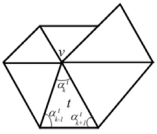
\includegraphics{fig/4.png}
% \end{wrapfigure}
\end{document}